\documentclass{standalone}
\usepackage{tikz}
\usepackage{ctex,siunitx}
\setCJKmainfont{Noto Serif CJK SC}
\usepackage{tkz-euclide}
\usepackage{amsmath,bbding}
\usetikzlibrary{patterns, calc}
\usetikzlibrary {decorations.pathmorphing, decorations.pathreplacing, decorations.shapes,}

\begin{document}
\small
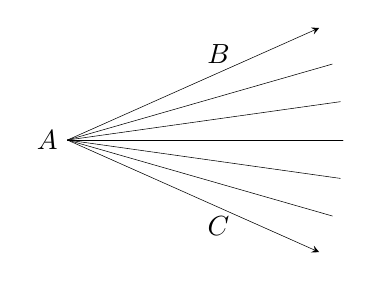
\begin{tikzpicture}[>=stealth,scale=0.7]
  \tkzSetUpPoint[fill=black]
  % \useasboundingbox(-1,-0.5)rectangle(1,0.5);
  \tkzDefPoints{0/0/A}
  \tkzDefShiftPoint[A](24:5){B'}
  \tkzDefShiftPoint[A](-24:5){C'}
  \tkzDefPointOnLine[pos=0.6](A,B')\tkzGetPoint{B}
  \tkzDefPointOnLine[pos=0.6](A,C')\tkzGetPoint{C}
  \foreach \x[count = \i] in {-16,-8,...,16}
  {
    \tkzDefShiftPoint[A](\x:5){P\i}
    \tkzDrawSegment(A,P\i)
  }
  \tkzDrawSegments[->](A,B' A,C')
  \tkzLabelPoints[below](C)
  \tkzLabelPoints[left](A)
  \tkzLabelPoints[above](B)
\end{tikzpicture}
\end{document}